
\section{El virus del dengue}

\subsection{Introducción}
El dengue es una enfermedad infecciosa causada por el virus del dengue transmitida por el mosquito Aedes Aegypti que puede ser mortal. La probabilidad de mortalidad puede verse reducida en 0.001 en el caso de ser tratado a tiempo.\\

Afecta a paises en regiones tropicales con climas calidos principalmente en zonas urbanas. La enfermedad causa sindromes gripales como fiebre, tos, dolor de cabeza, resfrio, dolor de garganta y musculos. La lucha contra el flagelo de la enfermedad depende de forma exclusiva de las medidas para controlar el vector que transmite la enfermedad, el mosquito Aedes Aegypti\\

El dengue hemorragico es mas comun en pacientes que ya han padecido la enfermedad con anterioridad. Existen diferentes serotipos de la enfermedad y en el caso de haber padecido un serotipo primario existe la posibilidad que ante un nuevo contagio se desarrolle otro serotipo lo cual derive en el padecimiento de caso de dengue hemorragico

\subsection{Epidemiología}

Durante la decada 2000 se ha visto un notable crecimiento de afectados de la enfermedad en la zona de america latina en paises como Paraguay, Brasil, Venezuela Peru. Principalmente en nuestro pais, Paraguay, existen epidemias  de distintos grados de gravedad en cada temporada de verano. Estas epidemias son ocasionadas principalmente por la falta de medidas de prevencion y control contra el mosquito transmisor Aedes Aegypti.\\

Si bien es cierto que se realizan campañas contra la enfermedad, los recorridos de fumigacion y limpieza terminan siendo obsoletos ante el no despertar ciudadano frente a la enfermedad. La existencia de grandes cantidades de patios baldios y terrenos sucios en zonas urbanas dificulta la eliminacion del agente transmisor y como consecuencia la enfermedad prevalece y se propaga.\\

La cantidad de afectados por la enfermedad en los ultimos años en todo Paraguay son:
\begin{itemize}
\item 13.766 casos en el año 2010
\item 42.945 casos en el año 2011
\item 2.347 casos en el año 2012
\item 130.155 casos en el año 2013\\
\end{itemize}

El aumento de la población del vector en zonas urbanas del pais, la masiva presencia del virus dengue en los países vecinos, la no colaboración de la poblacion para la eliminacion de criaderos de mosquitos de Aedes aegypti, además de la gran circulación de la poblacion en entre zonas habitadas son alguno de los factores que permiten que la enfermedad siga provocando olas de alerta y riesgo. A estos factores hay qye sumar el factor de la temperatura de nuestro país que es ideal para el desarrollo del agente transmisor.\\


Uno de los objetivos criticos es proveer un sistema de informacion que permita accionar preventivo en zonas de posibles focos de la enfermedad. Cada año en las ultimas 2 decadas se revive la misma situacion, hospitales abarrotados, escases de medicos y medicamentos, situacion de alerta, colapso social ante la epidemia.\\

\subsection{Distribucion Geografica}

El dengue es una enfermedad presente en todo el territorio del Paraguay con fuerte presencia desde hace una decada. Pero la distribucion de la enfermedad no es homogenea sino que se mapea a nivel macro a la distribucion de la poblacion. De ahí que el departamento central es uno de los departamentos con mayor indice de infestación de la enfermedad. En la figura 1 se obserba el resumen de los primeros meses del 2014. Departamentos clasificados segun sean zonas endemicas o no. Los departamentos con mayor densidad poblacional y movimiento de personas son siempre zonas endemicas.\\

Las zonas más afectadas en nuestro país son los departamentos de Central, Amambay e Itapúa. Seguidos de Coordillera, Paraguari y Alto Parana. Otras zonas y departamentos también presentan casos de la enfermedad solo que no son consideradas zonas endemicas o de riesgo. Esta distribución que denota las zonas de mayor riesgo se repite en cada época de flagelo de la enfermedad.\\

A nivel intrinseco en los objetivos de este trabajo está realizar resumenes en mapas similares a los que se muestran en las figuras 1, 2 y 3 pero conteniendo informacion a priori sobre la enfermedad. No señalar las zonas endemicas o no endemicas sino señalar las posibles zonas endémicas o no endémicas según información recolectada sobre la distribución larvaria. Esto permitiría realizar planes de control y prevención de la enfermedad.\\

\begin{figure}
\centering
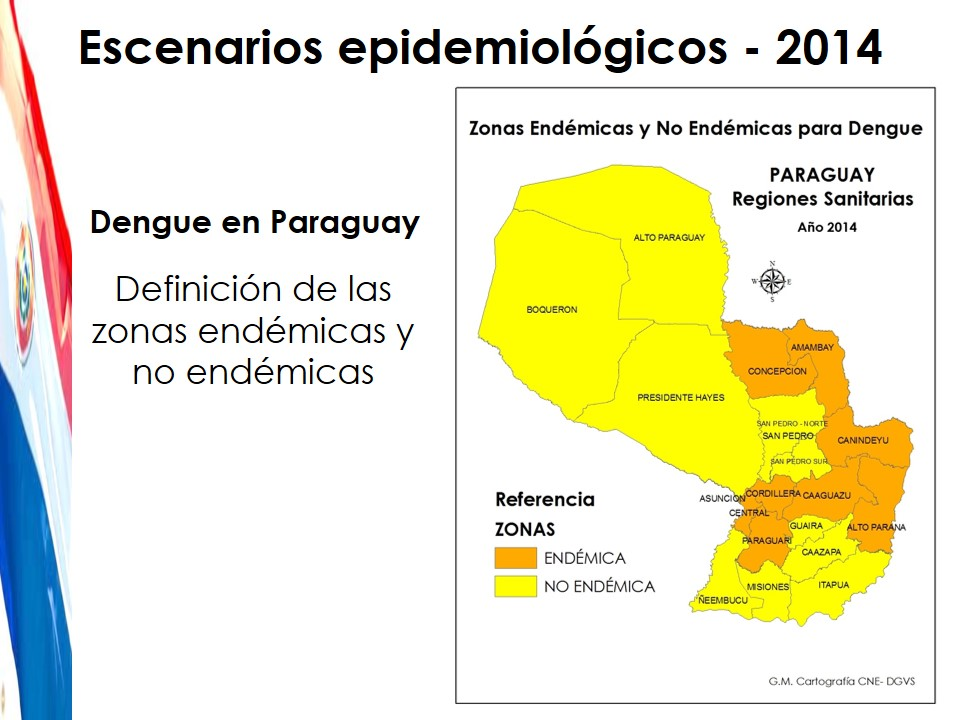
\includegraphics[width=0.8\textwidth]{./graphics/Diapositiva03.JPG}
\caption{\label{fig:mapa1}Zonas endemicas en todo el pais. Anho 2014}
\end{figure}

\begin{figure}
\centering
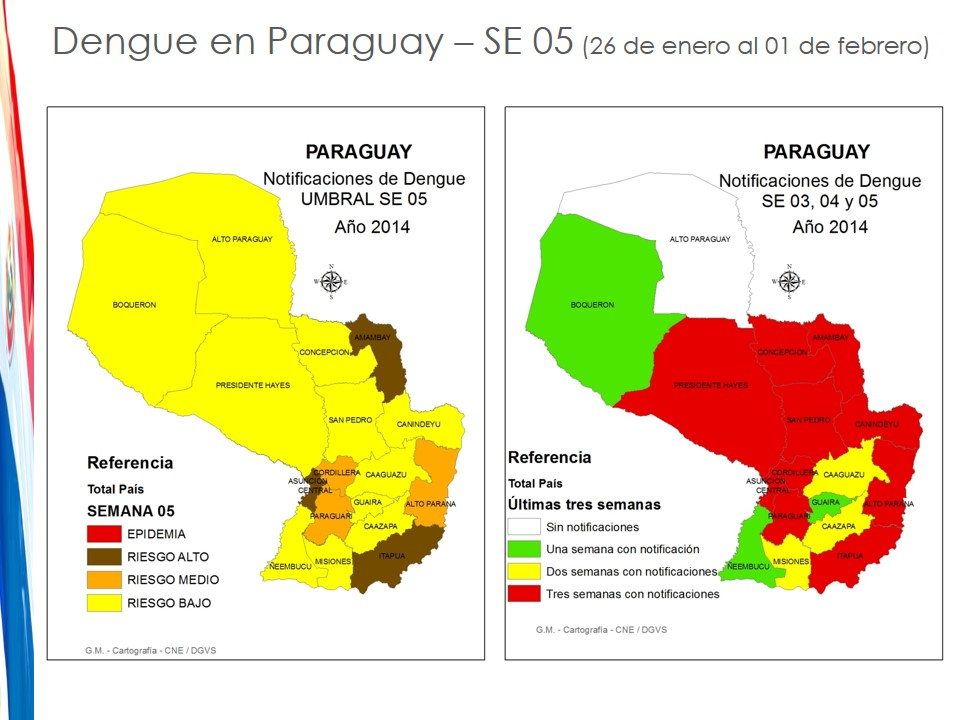
\includegraphics[width=0.8\textwidth]{./graphics/Diapositiva04.JPG}
\caption{\label{fig:mapa2}Mapa de riesgo de la semana epidermiologica 05. Anho 2013 }
\end{figure}

\begin{figure}
\centering
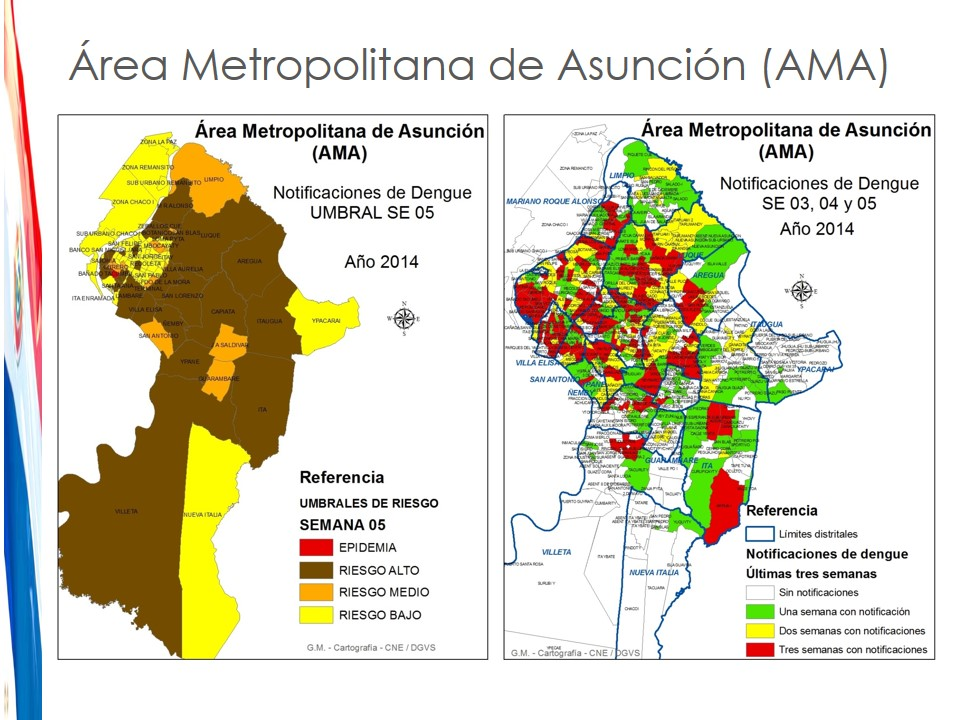
\includegraphics[width=0.8\textwidth]{./graphics/Diapositiva05.JPG}
\caption{\label{fig:mapa3}Mapa del area metropolitana de Asuncion.}
\end{figure}

\subsection{Salud publica}
Cada año el ministerio de salud pública y bienestar social (MSPyBS) en conjunto con otras organizaciones estatales y privadas realiza un plan de de acción en contra de la enfermedad. Un documento detallado presenta el proyecto y los responsables de llevarlo a cabo. El problema de los planes de acción es la dependencia del accionar ciudadano.
Del documento Dengue Plan 12 11 13 del MSPyBS se menciona los objetivos del plan de acción: \\

\textit{"...Los objetivos específicos para cada pilar son los siguientes:\\
\begin{enumerate}
\item Coordinación y Planificación: Fomentar el trabajo intersectorial, el monitoreo y la difusión del plan de acción
\item Vigilancia Entomológica: Vigilar, informar y alertar sobre riesgos ambientales
\item Control Vectorial: Disminuir la población de mosquitos
\item Vigilancia Laboratorial: Garantizar la representatividad de la vigilancia
\item Laboratorio de apoyo en Servicios: Garantizar el acceso a pruebas laboratoriales de diagnóstico
\item Vigilancia Epidemiológica: Aumentar la sensibilidad y oportunidad de la vigilancia
\item Componente Ambiental: Promover intervenciones sobre determinantes de la presencia del mosquito
\item Promoción y Participación Social: Fomentar la movilización social en acciones de control y prevención
\item Comunicación: Informar a la población sobre la problemática del dengue
\item Atención Integral: Asegurar la atención adecuada y oportuna a las personas con síndrome febril agudo con sospecha de dengue..."
\end{enumerate}}

Se concluye de los objetivos la dependencia del accionar de la población. Sin el apoyo de la ciudadanía no es posible controlar el vector ni realizar una vigilancia efectiva . La participación ciudadana tiene que empezar desde el conocimiento de la enfermedad y del vector transmisor. A eso debe sumarse la predisposición para realizar la limpieza del hogar/es propios mediante la eliminación de recipientes que acumulen agua principalmente. El problema es la enorme cantidad de patios baldíos y terrenos desabitados que luego de lluvias terminan siendo sitios propensos para alojar al mosquito.\\


La propuesta realizada en este trabajo tambíén requiere de la participación de la ciudadanía, pero desde un punto de vista distinto ya que el plan de acción será aplicado a las zonas de alto índice de población larval en primer lugar, permitiendo optimizar recursos y fuerza. Requerir de la acción ciudadana luego de que se presenten casos de la enfermedad se torna imposible, el estado de alerta desata preocupación y poco interés en luchar contra la enfermedad. La población en caso de riesgo busca refugiarse del la ola de la enfermedad y aunque existe colaboración para realizar un control sobre el vector el hecho de que ya exista afectados impide lograr una lucha eficiente.

\section{Aedes Aegypti. Mosquito transmisor del dengue}
El Aedes Aegypti  es el principal transmisor de la enfermedad del dengue. Es un mosquito que tiene como principales caracteristicas su contextura oscura y pequeña y sus manchas blancas en las extremidades. Mide apróximadamente 5mm. Al igual, evidentemente, que la enfermedad del dengue el mosquito se encuentra en zonas urbanas de regiones y paises tropicales.\\

Se estima que el mosquito causa mas de 50 millones de infecciones y mas de 26.000 muertes por año
Se recomiendan como metodo preventivo la utilizacion de repelentes que contengan DEET ya que son considerados como el mejor repelente contra el mosquito\\

\subsection{Biología}

El ciclo de vida del Aedes Aegypti es comun como otros mosquitos de especies similares. Basicamente consta de 4 estados:\\
\begin{itemize}
\item Huevo
\item Larva
\item Pupa
\item Adulto\\
\end{itemize}

Los huevos son depositados en las paredes de los recipientes por encima del nivel del agua. Los mismos son resitentes a temporadas de sequías largas. El contacto del agua con los huevos el paso a la siguiente etapa del mostiquito.\\

Los huevos eclosionan y pasan al estado de larvas. Las larvas son individuos móviles que se alimentan de residuos orgánicos encontrados en las paredes y fondos de los recipientes que los contienen. El paso a la siguiente etapa depende de la cantidad de alimentos, la temperatura y la densidad de larvas en el recipiente. Si se dan las condiciones se produce la metamorfosis y pasa al estado de pupa.\\

Las pupas no se alimentan, flotan en la superficie hasta alcanzar el estado adulto en aproximadamente 2 a 4 dias. El tiempo total de huevo a adulto es entre 7 a 14 dias. El tiempo es variable segun la duracion de cada cambio de estado.\\

El adulto se alimenta del nectar y aceites de plantas, pero la hembra del aedes aegipty necesita alimentarse de sangre para la formacion de los huevos y lo hace atravez de cualquier vertebrado teniendo preferencia por el humano.\\

Sus hábitos alimenticios pueden describirse por franjas horarias ya que se alimentan al amanecer y al atardecer. Buscan lugares oscuros de donde emerger y atacan a la victima en la piel cualquier parte del cuerpo  descubierta. Son muy habituales las picaduras en las manos, brazos, cuello, piernas. El contagio se produce cuando el mosquito hembra se alimenta de sangre humana infectada con el virus y luego pica a otro humano. No puede transmitirse de forma directa entre humano y humano\\

Su habitat para reproduccion y ovipostura son los lugares con agua estancada preferentemente limpia, lugares oscuros y quietos tales como latas, botellas vacías, neumáticos usados, baldes, etc.\\

\subsection{Cambios Climáticos}

Uno de los aspectos más importantes del mosquito Aedes Aegypti es su dependencia a la temperatura. Un país con temperatura tropical (promedio 25º C.) es un país ideal para la supervivencia del Aedes Aegypti no así un país con extremo calor o un clima más frío. Cada etapa de su desarrollo está ligado a condiciones climáticas; no solo temperatura sino también, lluvias y humedad. La lluvia permite que el agua se acumule en distintos recipientes; barriles, llantas y cubiertas, planteras, canaletas, etc. Se realizaron varios estudios analizando la influencia de la temperatura en el desarrollo del mosquito Aedes Aegypti. De los resultados de las pruebas se pueden obtener datos como el promedio de días en el que se pasa del estado larva a pupa ver Cuadro 1.\\

Esta información es muy valiosa en el estudio del mosquito ya que con el pronóstico del tiempo uno puede estimar el tiempo de desarrollo del Aedes Aegypti y determinar el crecimiento de la población actual (por ej. En 15 días aumentará la población actual del Aedes Aegypti en un 20\% dada las condiciones del clima previsto en esta zona)

\subsection{Ciclo gonadotrófico}
Después de cada alimentación se desarrolla un lote de huevos. Si la hembra completa su alimentación sanguínea (2-3 mg) desarrollará y pondrá 100-200 huevos, el intervalo dura de dos a tres días. La hembra grávida buscará recipientes oscuros o sombreados para depositar sus huevos, prefiriendo aguas limpias y claras.\\

\subsection{Rango de vuelo}
La hembra no sobrepasa los 50-100 m durante su vida (puede permanecer en la misma casa donde emergió). Si no hay recipientes, una hembra grávida puede volar tres kilómetros para poner sus huevos. Los machos se dispersan menos que las hembras.\\

\subsection{Conducta de reposo}
Descansan en lugares sombreados como alcobas, baños, patios o cocinas. Se les captura sobre ropas colgadas, debajo de muebles, toallas, cortinas y mosquiteros.\\

\subsection{Longevidad}
Los adultos pueden permanecer vivos en el laboratorio durante meses y en la naturaleza pocas semanas. Con una mortalidad diaria de 10\%, la mitad de los mosquitos morirán durante la primera semana y 95\% en el primer mes.\\


\begin{table}
\centering
\begin{tabular}{l|r}
Temperatura & Tiempo en estado larval y pupa \\\hline
13 & 0 \\
15-20 & 10 a 17.4 \\
20-25 & 9 a 13 \\
25-36 & 5 a 7 \\
36+ & 0
\end{tabular}
\caption{\label{tab:widgets}Tiempo promedio de duración en días del estado larval y pupa a diferentes temperaturas.}
\end{table}
